The previous section introduced the RF modules involved in the communication between the PCD and the PICC. This section will describe in detail each module of the analog front-end for ISO/IEC 14443A (see Fig. \ref{fig:afe}) and values of the components are shown in tables \ref{trans_specs} and \ref{res_specs}.

\begin{figure}[]
  \centering
  \includegraphics[page=10,width=90mm]{images-crop.pdf}
  \caption{PICC Analog Front-end}
  \label{fig:afe}
\end{figure}

\subsection{Power Supply Generator (PSG)}

The Power Supply Generator is divided into two parts: signal rectification and power limitation.

The first part rectifies the RF field signal and powers the chip. A full NMOS bridge rectifier \cite{rfid_rect1}\cite{rfid_rect2} was implemented in this design. The second part is a Shunt resistor that limits the voltage of the antenna and protects the whole chip. ISO/IEC14443-2 requires the PICC to work when magnetic intensity is between 1.5-7.5A/m rms. Therefore the PICC must be able to work under these extreme conditions.  

The simplified schematic of signal rectification is shown in Fig. \ref{fig:rect} and power limitation (Shunt resistor) is shown in Fig. \ref{fig:shunt}. The Shunt Resistor switches on at 2.6V using the components in tables \ref{trans_specs} and \ref{res_specs} and the simulation is shown in Fig. \ref{fig:shunt_sim}.

\begin{figure}[h]
  \centering
  \includegraphics[page=11,width=50mm]{images-crop.pdf}
  \caption{NMOS Bridge Rectifier}
  \label{fig:rect}
\end{figure}

\begin{figure}[h]
  \centering
  \includegraphics[page=12,width=50mm]{images-crop.pdf}
  \caption{Shunt Resistor}
  \label{fig:shunt}
\end{figure}

\begin{figure}[h]
  \centering
  \includegraphics[page=22,width=90mm]{images-crop.pdf}
  \caption{Shunt Resistor simulation}
  \label{fig:shunt_sim}
\end{figure}

\subsection{Clock Generator (CG)}

The Clock Generator gets the clock from the antenna and it is then used by the DPU. This module generates a 13.56MHz clock source. It consists of two D-Type Flip-Flops (Divide-by-2 clock signal) and an XOR logic gate. 

The phase difference between RF+ and RF- is 180 degrees, making it quite easy to recover the clock. The simplified schematic is shown in Fig. \ref{fig:clk} and the simulation in Fig. \ref{fig:clk_sim}.

A frequency divider by 4 is placed at the output of the clock generator. Reducing the work frequency also reduces the power consumed. On the other hand, a Carrier-Frequency/4 (3.39MHz) is used for the DPU, because the FDT (Frame Delay Time) defined in ISO/IEC14443-3 for all commands is a divisor of this frequency.
 

\begin{figure}[]
  \centering
  \includegraphics[page=13,width=90mm]{images-crop.pdf}
  \caption{Clock Generator schematic}
  \label{fig:clk}
\end{figure}

\begin{figure}[h]
  \centering
  \includegraphics[page=21,width=90mm]{images-crop.pdf}
  \caption{Clock recovery simulation}
  \label{fig:clk_sim}
\end{figure}


\subsection{Voltage Regulator (VR)}

The Voltage Regulator \cite{rfid_ldo} regulates the voltage supplied from PSG and provides a constant DC voltage at the output of this module. The VR is known as the series pass regulator, as shown in Fig. \ref{fig:ldo}. It consists of three major parts. An operational amplifier (OP-AMP) is used as error amplifier. A series pass transistor is used as a current amplifier. R3 and R4 are used as a resistive voltage divider (Equation \ref{eq:vref}). The reference voltage source Vref, in this case, is a beta multiplier \cite{panadero}. The power consumption of the VR is 3.5uA in simulation. 

\begin{equation} \label{eq:vref}
VDD = Vref*(1+R3/R4)
\end{equation}
%$$VDD = Vref*(1+R1/R2)$$  

%Basically it consist of a reference source, in this case, a beta multiplier is used for this purpose. The OP AMP play the role of controller, it copies the reference voltage, control the variation of VRECT or VDD and reflects the reference voltage to the output.

\begin{figure}[]
  \centering
  \includegraphics[page=15,width=70mm]{images-crop.pdf}
  \caption{Voltage Regulator schematic}
  \label{fig:ldo}
\end{figure}

\subsection{Modulator}

The modulator \cite{rfid_modulador} carries the signal from the PICC to the PCD module. There are two different types of load modulation: resistive and capacitive modulation. Both types create a subcarrier next to 13.56MHz. The NMOS transistors are switched on and off in time with the encoded data. This varies the load (resistive) or resonance frequency  (capacitive) of the transponder.  Resistive modulation was adopted in this design for its simplicity. The schematic is shown in Fig. \ref{fig:mod}.

\begin{figure}[h]
  \centering
  \includegraphics[page=16,width=40mm]{images-crop.pdf}
  \caption{Modulator schematic}
  \label{fig:mod}
\end{figure}

\subsection{Demodulator}

The demodulator recovers the digital frame transmitted from the PCD module. An Envelope Extractor (EE) circuit \cite{rfid_demodulador} is needed to extract the data. The digital signal is recovered by connecting the output of the EE with the input of the buffer. The circuit is shown in Fig. \ref{fig:demod}. 

\begin{figure}[h]
  \centering
  \includegraphics[page=17,width=70mm]{images-crop.pdf}
  \caption{Demodulator schematic}
  \label{fig:demod}
\end{figure}

\subsection{Power On Reset (POR)}

The Power On Reset module is used to reset the digital machine and put it into an idle state. It consists of a RC low pass network. When the chip enters the RF field, the VR turns on and powers all modules. The POR module holds the voltage of the VR and delays it. This signal is applied to the reset pin of the Flip-Flops in the digital machine. The schematic is shown in Fig. \ref{fig:por}. 

\begin{figure}[h]
  \centering
  \includegraphics[page=18,width=30mm]{images-crop.pdf}
  \caption{POR schematic}
  \label{fig:por}
\end{figure}


\begin{table}[h]
\centering
\caption{Transistors}
\label{trans_specs}
\begin{tabular}{c|c|c|c|c}
\textbf{Type}  & \textbf{Symbol}& \textbf{W}  & \textbf{L}  & \textbf{Fingers/Multiplicity}  \\ \hline
NMOS                 & Q1,Q2,Q3,Q4    & 10 um       & 0.4 um      & 20                \\
PMOS                 & Q5,Q6,Q7       & 5 um        & 0.4 um      & 1                 \\
NMOS                 & Q8             & 5 um        & 0.4 um      & 2                 \\
PMOS                 & Q9             & 15 um       & 0.4 um      & 25                \\
PMOS                 & Q10,Q11        & 1 um        & 3 um        & 2                 \\
NMOS                 & Q12,Q13        & 2 um        & 1 um        & 2                 \\
NMOS                 & Q14            & 0.5 um      & 3 um        & 1                 \\
PMOS                 & Q15            & 10 um       & 0.4 um      & 10                \\
NMOS                 & Q16,Q17        & 5 um        & 0.4 um      & 1                 \\
NMOS                 & Q18,Q19        & 3 um        & 0.4 um      & 10                \\
\end{tabular}
\end{table}

\begin{table}[h]
\centering
\caption{Additional Components}
\label{res_specs}
\begin{tabular}{c|c}
\textbf{Symbol} & \textbf{Value} \\ \hline
R1              & 10 k           \\
R2              & 48.5 k         \\
R3,R4           & 343 k          \\
R5,R6           & 37.5 k         \\
R7,R8           & 370            \\
R9              & 150 k           \\
C1              & 5p             \\
C2              & 3.5 p          \\
C3              & 7.8 p          \\


\end{tabular}
\end{table}